\section{2K Analysis (90 pts)\label{sec:6}}

    In this section a 2k3 analysis is performed on throughput and response time for experimental parameters listed in
    table \ref{tab:6_setup} using single keys for GET requests. In a 2k analysis factors are used as parameters
    to infer system behaviour. Table \ref{tab:6_2k-factors} lists these factors and their interpretation as per sign
    table.

    \begin{table}
        \scriptsize{
            \begin{tabular}{|l|c|}
                \hline Number of servers                & 1 and 3 \\
                \hline Number of client machines        & 3 \\
                \hline Instances of memtier per machine & 1 (1 middleware) or 2 (2 middlewares) \\
                \hline Threads per memtier instance     & 2 (1 middleware) or 1 (2 middlewares) \\
                \hline Virtual clients per thread       & 32 \\
                \hline Workload                         & Write-only and Read-only \\
                \hline Multi-Get behavior               & N/A \\
                \hline Multi-Get size                   & N/A \\
                \hline Number of middlewares            & 1 and 2 \\
                \hline Worker threads per middleware    & 8 and 32 \\
                \hline Repetitions                      & 3 or more (at least 1 minute each) \\
                \hline
            \end{tabular}
        \caption{Experimental parameters for 2k analysis.\label{tab:6_setup}}
        }
    \end{table}

    \begin{table}
        \small{
            \begin{tabular}{r l l l }
                \toprule
                Sign & Number of \srv{}s (\textbf{A}) & Number of \mw{}s (\textbf{B}) & Number of worker threads (\textbf{C})   \\
                \midrule
                -1  & 1                            & 1                           & 8   \\
                1   & 3                            & 2                           & 32  \\
                \bottomrule
            \end{tabular}
            \caption{Sign table interpretation with respective configuration value.\label{tab:6_2k-factors}}
        }
    \end{table}

    For 2k analysis two models exist, the additive and multiplicative one. Considering the factors to analyse, it
    becomes clear that increasing \textbf{A} and either \textbf{B} or \textbf{C}, an additive relationship exists
    whereas increasing \textbf{B} and \textbf{C}, a multiplicative relationship exists (due to being bound together). A
    mixed model would therefore be optimal. Due to an unavailability of one and with more factors being additive the
    additive model is used for analysis.

    \begin{table}
          \def\sym#1{\ifmmode^{#1}\else\(^{#1}\)\fi}%
        \footnotesize{
            \centering
            \begin{subfigure}[t!]{0.45\textwidth}
                \centering
                \begin{tabular}{l*{4}{c}}
                    \toprule
                    & \multicolumn{2}{c}{Throughput}  & \multicolumn{2}{c}{Response Time} \\
                    \cmidrule(lr){2-3}\cmidrule(lr){4-5}
                    & \multicolumn{1}{c}{Effect} & \multicolumn{1}{c}{Variation} & 
                      \multicolumn{1}{c}{Effect} & \multicolumn{1}{c}{Variation} \\
                    \midrule
                    q0            & 5694 & \textemdash & 44.1  & \textemdash \\
                    \addlinespace
                    qA            & 2760 & 98.24\%     & -21.2 & 99.73\% \\
                    qB            & 173  & 0.39\%      & -0.5  & 0.05\% \\
                    qC            & 139  & 0.25\%      & -0.4  & 0.04\% \\
                    \addlinespace
                    qAB           & 174  & 0.39\%      & -0.5  & 0.06\% \\
                    qAC           & 136  & 0.24\%      & -0.4  & 0.04\% \\
                    qBC           & -136 & 0.24\%      & -0.4  & 0.04\% \\
                    \addlinespace
                    qABC          & -135 & 0.24\%      & 0.4   & 0.03\% \\
                    \addlinespace
                    Error         & \textemdash & 0.01\% & \textemdash & 0.00\% \\
                    \bottomrule
                \end{tabular}
                \caption{2k3 factors for GET requests.\label{tab:6_get-factors}}
            \end{subfigure}
            \hspace{4em}
            \begin{subfigure}[t!]{0.45\textwidth}
                \centering
                \begin{tabular}{l*{4}{c}}
                    \toprule
                    & \multicolumn{2}{c}{Throughput}  & \multicolumn{2}{c}{Response Time} \\
                    \cmidrule(lr){2-3}\cmidrule(lr){4-5}
                    & \multicolumn{1}{c}{Effect} & \multicolumn{1}{c}{Variation} & 
                      \multicolumn{1}{c}{Effect} & \multicolumn{1}{c}{Variation} \\
                    \midrule
                    q0            & 7774 & \textemdash & 26.4 & \textemdash \\
                    \addlinespace
                    qA            & -573 & 7.87\%      & 2.1  & 9.55\% \\
                    qB            & 1149 & 31.56\%     & -3.9 & 32.81\%\\
                    qC            & 1530 & 55.93\%     & -5.0 & 54.85\% \\
                    \addlinespace
                    qAB           & 171  & 0.70\%      & -1.0 & 2.41\% \\
                    qAC           & -177 & 0.75\%      & -0.0 & 0.00\% \\
                    qBC           & 340  & 2.77\%      & 0.2  & 0.17\% \\
                    \addlinespace
                    qABC          & 115  & 0.32\%      & -0.2 & 0.11\% \\
                    \addlinespace
                    Error         & \textemdash & 0.09\% & \textemdash & 0.10\% \\
                    \bottomrule
                \end{tabular}
                \caption{2k3 factors for SET requests.\label{tab:6_set-factors}}
            \end{subfigure}
        \caption{2k3 factor analysis summaries for GET and SET requests.\label{tab:6_factor-analysis}}
        \vspace*{-0.75\baselineskip}
        }
    \end{table}

    In the case of GET packets the factor \textbf{A} is with nearly 100\% variational effect for throughput and
    response time the only relevant factor in determining the system behaviour. Of interesting note is the switch in
    sign yet including the interpretation that high throughput implies low response times it becomes apparent why a
    change in sign must happen for corresponding factors. As previously observed we see for three \cli{}s and one
    \srv{} immediately a saturation point and the middleware has no measurable effect, either good or bad on the
    system performance for GET. This matches the results observed. Visualizing the residuals (Figure
    \ref{fig:6_r_get_tp}) and doing a QQ plot (figure \ref{fig:6_qq_get_tp}) of the measured data for the
    throughput and response time (the latter omitted for behaving similar to the former) shows very consistent
    behaviour at either ends of the request throughputs on the residual plot. A few outliers are observed but these
    cannot be ruled out in a cloud environment. The QQ plot has a very shallow line in the center where the highest
    likelihood of an observation is for a standard distribution. This shows a good fit of the additive model.

    In the case of SET requests a mixture of factors \textbf{C} and \textbf{B} shows to be mostly significant with
    around 55.9\%/54.9\% and 31.6\%/32.8\% for throughput and response time respectively. Of minor significance yet
    measurable are \textbf{A} with around 7.8\%/9.6\% for throughput and response time and \textbf{BC} for
    throughput with 2.8\% (which interprets as increasing the number of \mw{}s and worker threads simultaneously).
    The change in sign occurs again correctly. The analysis aligns with previous observations and conclusions while
    bringing up the hypothesis that worker threads result in a larger gain in performance compared to adding more
    \mw{}s. The hypothesis seems to not hold though as in Experiment 3 we expect for the case of two \mw{}s and 16
    worker threads less performance than for one \mw{} and 32 worker threads. This is clearly not the case and as
    such the belief is the model is unable to correctly differentiate between these two parameters (assuming both
    \mw{}s have the exact same throughput and response time behaviour). The factor \textbf{A}, adding more \srv{}s to
    the system, does align with results from experiments \ref{sec:3} and \ref{sec:4} where the number of \srv{}s changes
    from one to three and a decrease in throughput is observed. The factor proposes an increase in \srv{}s introduces a
    negative effect as the \mw{} is designed to share the SET operation with each \srv{} in the system. This key
    distribution introduces additional latencies into the system. Again residual (figure \ref{fig:6_r_set_tp}) and QQ
    plots (figure \ref{fig:6_qq_set_tp} were created but only the throughput ones are presented (similar behaviour in
    either case). The residuals are scattered without anything being possible to interpret and the QQ plot shows a
    quasi-linear behaviour. It can be concluded that the additive model is insufficient to model the behaviour as the
    distribution is uniform and seems to follow no trend. The numbers still show a trend but their expressiveness is
    uncertain.

    \begin{figure*}
        \vspace*{-.5\baselineskip}
            \centering
        \begin{subfigure}[t!]{0.45\textwidth}
            \centering
            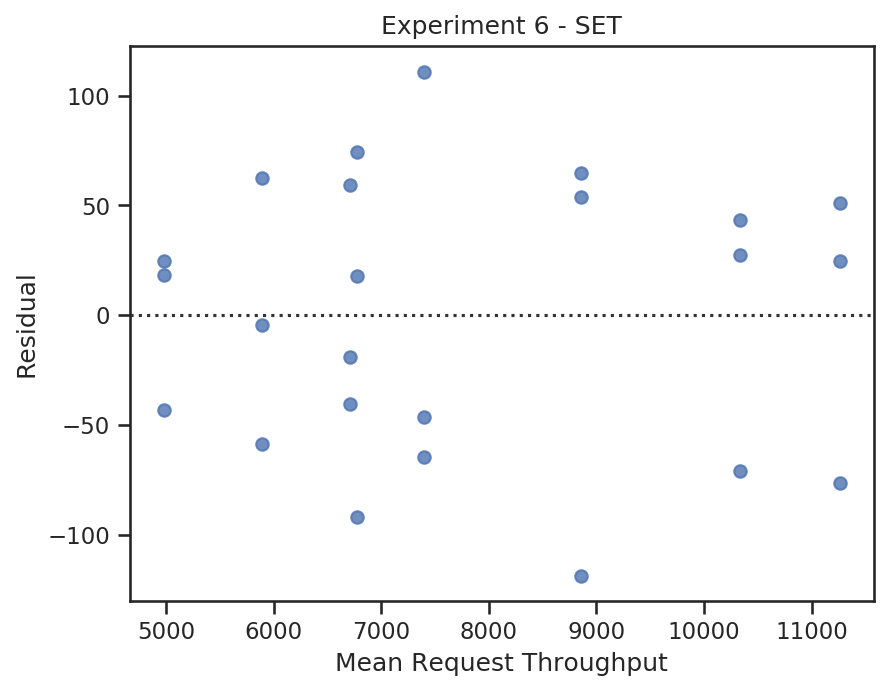
\includegraphics[width=\textwidth]{../data_analysis/figures/6-0_throughput-set-residual.png}
            \caption{Residual plot for SET Throughput.\label{fig:6_r_set_tp}}
            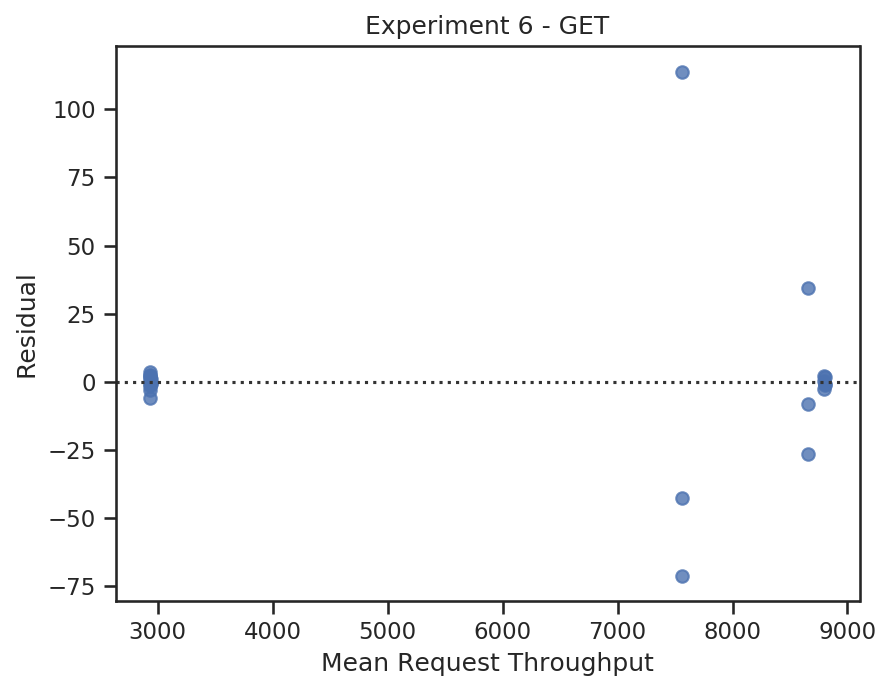
\includegraphics[width=\textwidth]{../data_analysis/figures/6-0_throughput-get-residual.png}
            \caption{Residual plot for GET Throughput.\label{fig:6_r_get_tp}}
        \end{subfigure}
        \begin{subfigure}[t!]{0.45\textwidth}
            \centering
            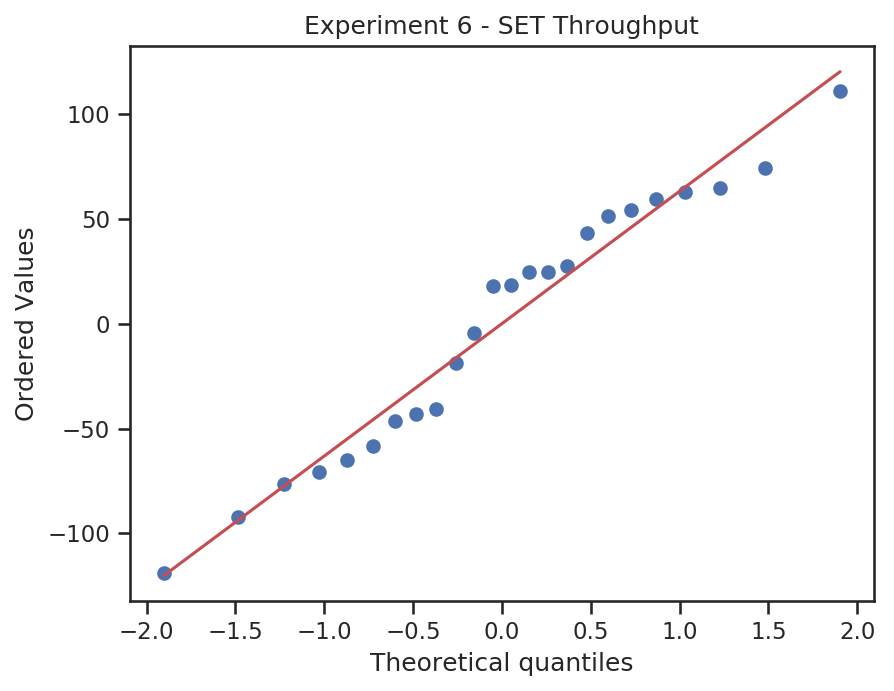
\includegraphics[width=\textwidth]{../data_analysis/figures/6-0_throughput-set-qq.png}
            \caption{QQ-Plot for SET Throughput.\label{fig:6_qq_set_tp}}
            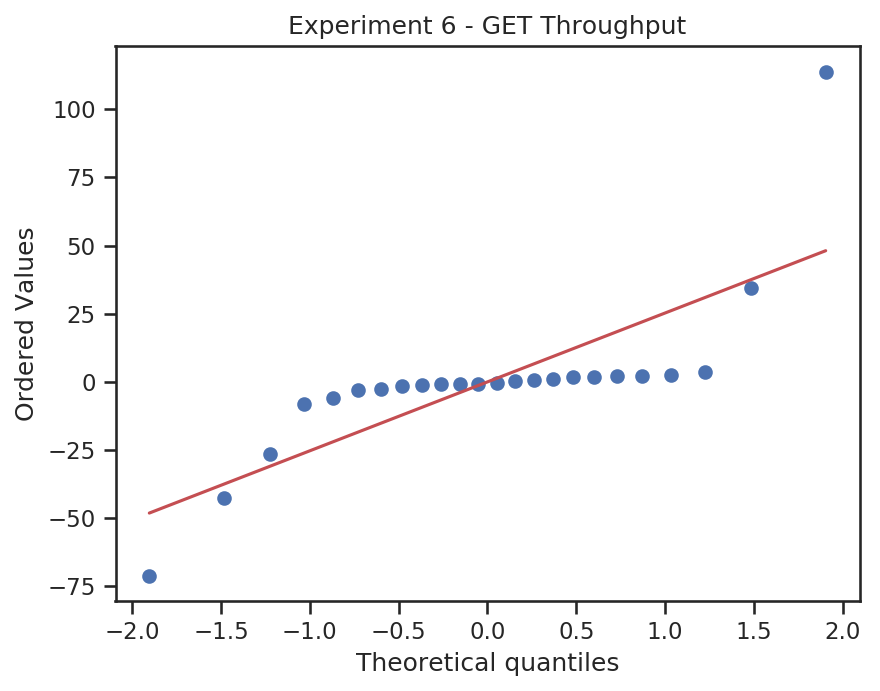
\includegraphics[width=\textwidth]{../data_analysis/figures/6-0_throughput-get-qq.png}
            \caption{QQ-Plot for GET Throughput.\label{fig:6_qq_get_tp}}
        \end{subfigure}
        \caption{Residual and QQ plots based on memtier measurements for Experiment 6.0. Throughput only plots
                 are depicted.\label{fig:6_tp}}
    \end{figure*}
